\documentclass[a4paper,11pt]{article}
\usepackage[portuguese]{babel}
\usepackage{graphicx}
\usepackage{amsmath}
\usepackage{minted}
\usepackage{mdframed}

\usepackage[twoside,verbose,body={16cm,24cm},
left=25mm,top=20mm]{geometry}


\title{Cálculo de Programas \\ Resolução - Ficha 01}
\author{Eduardo Freitas Fernandes}
\date{2025}

\setminted{
	frame=single,
	tabsize=4,
	breaklines=true
}


\begin{document}
	
\maketitle
	
\noindent \underline{\textbf{Exercício 1}}\\

\begin{minipage}{0.45\textwidth}
\begin{mdframed}
	\[
	\begin{aligned}
		\pi_1 \cdot (f \times g) \  (x, y) 
		= \  &\{\text{def. composição}\}\\
		&\pi_1 ((f \times g) (x, y)) \\
		= \  &\{\text{(F1)}\}\\
		&\pi_1 (f \  x, g \  y) \\
		= \  &\{\text{(F2)}\}\\
		&f \  x \\
		= \  &\{\text{(F1)}\}\\
		&f (\pi_1 (x, y)) \\
		= \  &\{\text{def. composição}\}\\
		&f \cdot \pi_1
	\end{aligned}
	\]
\end{mdframed}	
\end{minipage}
\hfill
\begin{minipage}{0.45\textwidth}
\begin{mdframed}
	\[
	\begin{aligned}
		\pi_2 \cdot (f \times g) \  (x, y) 
		= \  &\{\text{def. composição}\}\\
		&\pi_2 ((f \times g) (x, y)) \\
		= \  &\{\text{(F1)}\}\\
		&\pi_2 (f \  x, g \  y) \\
		= \  &\{\text{(F2)}\}\\
		&g \  y \\
		= \  &\{\text{(F1)}\}\\
		&g (\pi_2 (x, y)) \\
		= \  &\{\text{def. composição}\}\\
		&g \cdot \pi_2
	\end{aligned}
	\]
\end{mdframed}
\end{minipage}

\begin{center}
\begin{minipage}{0.5\textwidth}
	\begin{mdframed}
		\[
		\begin{aligned}
			(f \times g) \  (x, y)
			= \  &\{\text{(F1)}\}\\
			&(f \  x, g \  y) \\
			= \  &\{\text{(F2)}\}\\
			&(f (\pi_1 (x, y)), g (\pi_2 (x, y))) \\
			= \  &\{\text{def. composição}\}\\
			&(f \cdot \pi_1, g \cdot \pi_2) \\
			= \  &\{\text{def. split}\}\\
			&\langle f \cdot \pi_1, g \cdot \pi_2 \rangle \\
		\end{aligned}
		\]
	\end{mdframed}
\end{minipage}
\end{center}


	\noindent \underline{\textbf{Exercício 2}}
	
	
	
	
	\noindent \underline{\textbf{Exercício 3}}
	
	
	
	
	\noindent \underline{\textbf{Exercício 4}}
	
	
	
	\noindent \underline{\textbf{Exercício 5}}
	\[
	\begin{aligned}
		\underbrace{\langle h, k\rangle \cdot f}_{k} &= \underbrace{\langle h \cdot f, k \cdot f \rangle}_{\langle h, f \rangle} \\
		\iff &\{\text{(F7)}\} \\
		&\begin{cases}
			\pi_1 \cdot \langle h, k \rangle \cdot = h \cdot f \\
			\pi_2 \cdot \langle h, k \rangle \cdot = k \cdot f \\
		\end{cases}\\
		\iff &\{\text{Cancelamento-$\times$}\} \\
		&\begin{cases}
			h \cdot f \\
			k \cdot f \\
		\end{cases}
	\end{aligned}
	\]
	
	
	
	\noindent \underline{\textbf{Exercício 6}}
	
	
	
	\noindent \underline{\textbf{Exercício 7}}
	
	
	
	\noindent \underline{\textbf{Exercício 8}}
	
	
	
	\noindent \underline{\textbf{Exercício 9}}
	
\begin{minted}{haskell}
acronym :: String -> String
acronym = map head . words

short :: String -> String
short = uncurry (++) . (id >< (' ':)) . split head last . words
\end{minted}

\begin{figure}[H]
	\centering
	\fbox{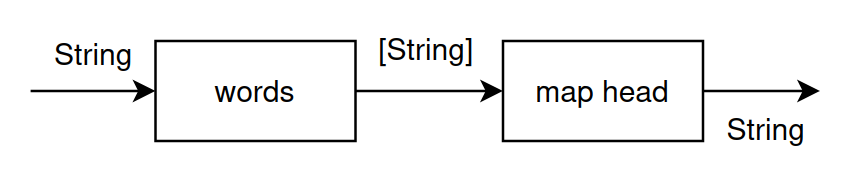
\includegraphics[width=0.4\textwidth]{imgs/acronym.png}}
	\caption{acronym}
\end{figure}
	
\begin{figure}[H]
	\centering
	\fbox{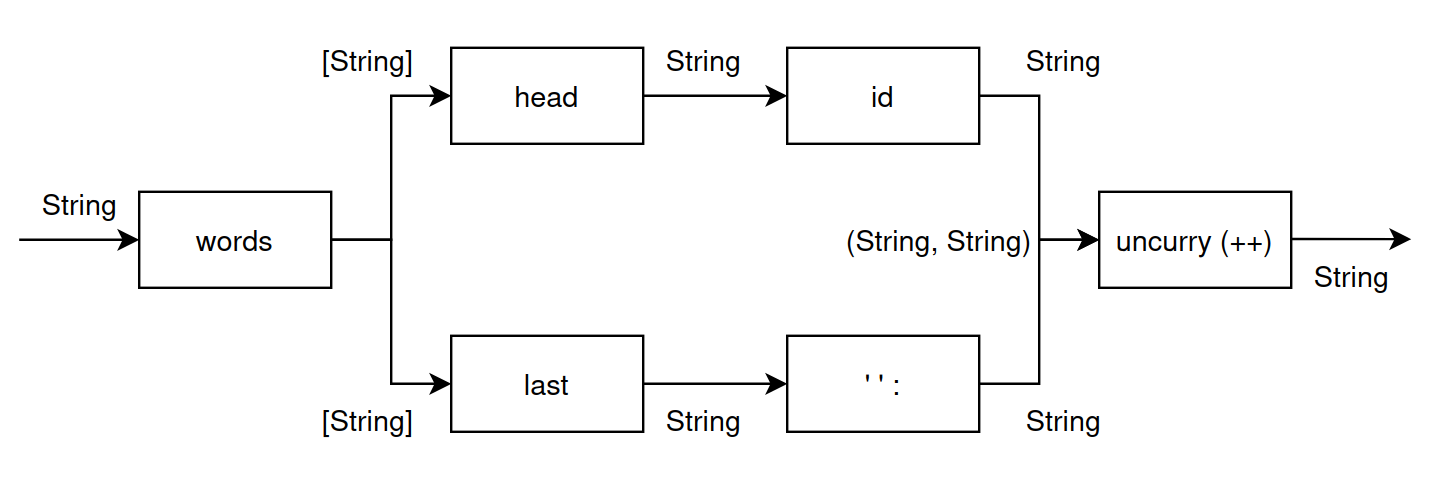
\includegraphics[width=0.6\textwidth]{imgs/short.png}}
	\caption{short}
\end{figure}

	
\end{document}
